\documentclass[aspectratio=169, 11pt]{beamer}

% ====== Theme ======
\usetheme{Madrid}
\definecolor{CityUBlue}{RGB}{0, 51, 102}
\definecolor{CityULightBlue}{RGB}{0, 102, 179}
\definecolor{CityUGold}{RGB}{198, 163, 0}
\usecolortheme[named=CityUBlue]{structure}
\setbeamercolor{title}{fg=white, bg=CityUBlue}
\setbeamercolor{frametitle}{fg=white, bg=CityUBlue}
\setbeamercolor{block title}{bg=CityUBlue, fg=white}
\setbeamercolor{block body}{bg=CityUBlue!10, fg=black}
\setbeamercolor{item}{fg=CityUBlue}
\setbeamercolor{subitem}{fg=CityULightBlue}

% ====== Packages ======
\usepackage[T1]{fontenc}
\usepackage{lmodern}
\usepackage{booktabs}
\usepackage{graphicx}
\usepackage{hyperref}
\usepackage{amsmath, amssymb}
\usepackage{tikz}
\usepackage{appendixnumberbeamer}

% ====== Settings ======
\setbeamertemplate{navigation symbols}{}
\graphicspath{{figures/}{../../Figures used in slides/}}

% ====== Metadata ======
\title[EF8083 Lecture 1]{PhD Lecture in Behavioral Asset Pricing:\\ Introduction}
\author[F.\ W.\ Li]{Frank Weikai Li}
\institute[CityU]{Associate Professor of Finance\\City University of Hong Kong}
\date{}

% ==============================================================================
\begin{document}
% ==============================================================================

% --- Slide 1: Title ---
\begin{frame}[plain]
\titlepage
\end{frame}

% --- Slide 2: Overview ---
\section{Overview}

\begin{frame}{Overview}
\begin{itemize}
\item \textbf{Definition 1:}
  \begin{itemize}
  \item Behavioural Finance investigates whether some financial phenomena are the result of less than fully rational thinking
  \end{itemize}
\item \textbf{Three paradigms in finance:}
\item Traditional finance
  \begin{itemize}
  \item Agents are rational and there are no frictions
  \end{itemize}
\item Frictional finance
  \begin{itemize}
  \item Agents are rational but there are frictions
  \end{itemize}
\item Behavioral finance
  \begin{itemize}
  \item Some agents are less than fully rational
  \end{itemize}
\end{itemize}
\end{frame}

% --- Slide 3: Overview, ctd. ---
\begin{frame}{Overview, ctd.}
\begin{itemize}
\item \textbf{Rationality means two things:}
  \begin{itemize}
  \item Update beliefs correctly on receipt of new information, i.e.\ according to Bayes' rule
  \item Make decisions according to sensible preferences, i.e.\ according to expected utility
    \begin{itemize}
    \item Where the utility function is defined over wealth or consumption
    \end{itemize}
  \end{itemize}
\item \textbf{In behavioural finance, then:}
  \begin{itemize}
  \item We study less than fully rational beliefs
    \begin{itemize}
    \item Deviations from Bayes' rule
    \end{itemize}
  \item And less than fully rational preferences
    \begin{itemize}
    \item Non-EU, or EU defined over things other than wealth or consumption
    \end{itemize}
  \end{itemize}
\end{itemize}
\end{frame}

% --- Slide 4: Overview, ctd. ---
\begin{frame}{Overview, ctd.}
\begin{itemize}
\item \textbf{Definition 2:}
  \begin{itemize}
  \item Behavioral finance tries to understand financial phenomena using models that are \emph{psychologically more realistic} than their predecessors
  \end{itemize}
\item \textbf{Three paradigms in finance:}
\item \textbf{Traditional finance}
  \begin{itemize}
  \item Very basic, psychologically and institutionally
  \end{itemize}
\item \textbf{Frictional finance}
  \begin{itemize}
  \item More realistic, institutionally
  \end{itemize}
\item \textbf{Behavioral finance}
  \begin{itemize}
  \item More realistic, psychologically
    \begin{itemize}
    \item More psychologically realistic assumptions about beliefs
    \item More psychologically realistic assumptions about preferences
    \end{itemize}
  \end{itemize}
\end{itemize}
\end{frame}

% --- Slide 5: Challenges ---
\begin{frame}{Challenges for Behavioural Finance}
\begin{itemize}
\item \textbf{The arbitrage critique}
  \begin{itemize}
  \item Claim: rational agents will quickly undo any effect irrational agents have on prices
    \begin{itemize}
    \item They will engage in ``arbitrage''
    \end{itemize}
  \item We now know that there are ``limits to arbitrage''
  \end{itemize}
\item \textbf{The lack-of-discipline critique}
  \begin{itemize}
  \item Claim: behavioural finance is ``underdisciplined''; it is too easy to find psychology that fits the facts
    \begin{itemize}
    \item Address this by testing new predictions
    \end{itemize}
  \end{itemize}
\end{itemize}
\end{frame}

% --- Slide 6: Lecture structure ---
\begin{frame}{Lecture Structure}
\begin{itemize}
\item \textbf{I.\ Introduction}
  \begin{itemize}
  \item Overview
  \item Facts
    \begin{itemize}
    \item Asset price
    \item Investor trading and portfolio choice
    \end{itemize}
  \end{itemize}
\item {\large \textbf{II.\ Limits to Arbitrage}}
\item \textbf{III.\ Psychological Foundation and Applications in Finance}
  \begin{itemize}
  \item Non-standard preferences
  \item Biased beliefs
  \item Heterogeneous beliefs
  \item Bounded rationality and psychology-free models
  \end{itemize}
\end{itemize}
\end{frame}

% --- Slide 7: Roadmap ---
\section{Aggregate Stock Market}

\begin{frame}{Roadmap}
\begin{itemize}
\item \textbf{Asset pricing}
  \begin{itemize}
  \item Aggregate stock market
  \item Cross-section of stock returns
  \item Other asset classes
  \item Bubbles
  \end{itemize}
\item \textbf{Investor trading and portfolio choice}
  \begin{itemize}
  \item Individual investors
  \item Institutional investors
  \end{itemize}
\end{itemize}
\end{frame}

% --- Slide 8: Aggregate stock market, ctd. ---
\begin{frame}{Aggregate Stock Market, ctd.}
\begin{columns}[T]
\begin{column}{0.52\textwidth}
\begin{itemize}
\item \textbf{The time-series predictability puzzle}
  \begin{itemize}
  \item Aggregate stock market returns are predictable in the time series
    \begin{itemize}
    \item E.g.\ by the price-dividend (P/D) or price-earnings ratio (P/E)
    \end{itemize}
  \item This seems to contradict efficient market hypothesis
  \end{itemize}
\end{itemize}
\end{column}
\begin{column}{0.46\textwidth}
\centering
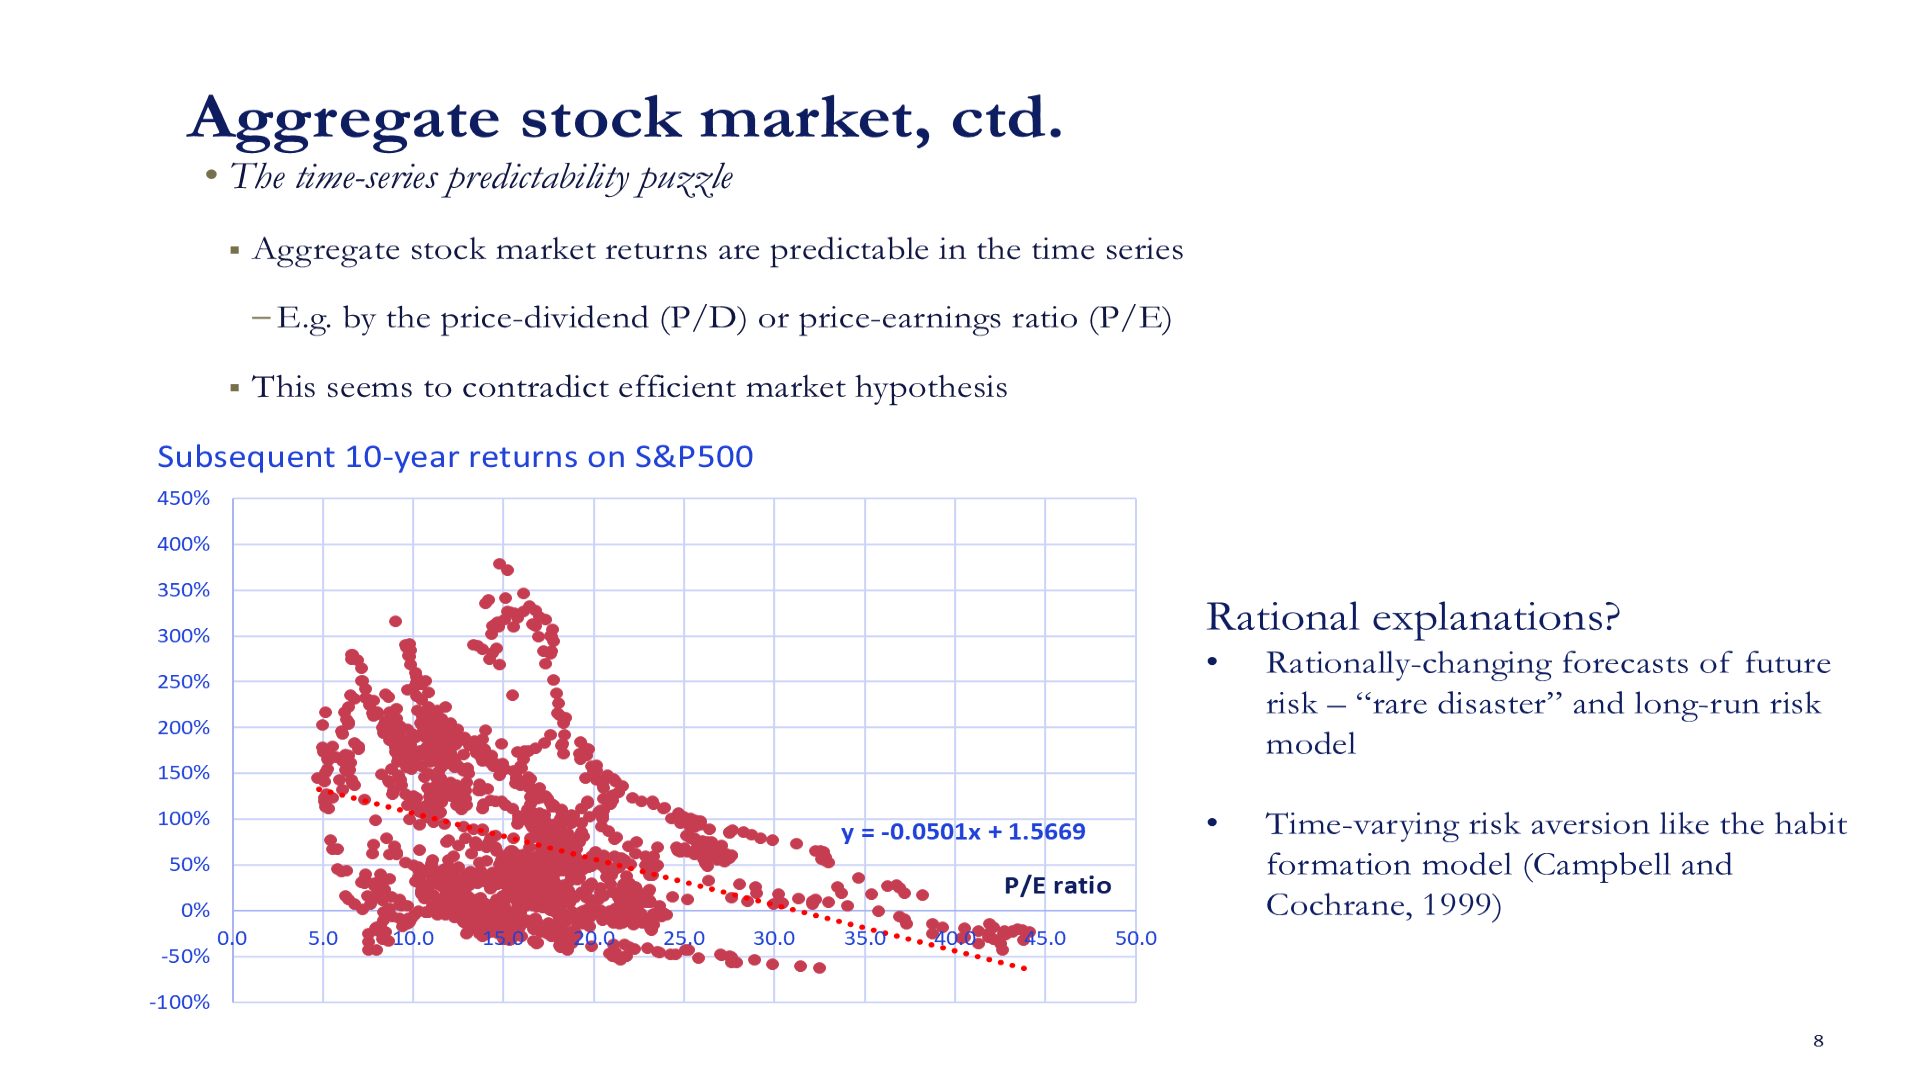
\includegraphics[width=\textwidth]{figures/slide08_chart.png}

\vspace{0.3em}
\footnotesize
\textbf{Rational explanations?}\\
Rationally-changing forecasts of future risk --- ``rare disaster'' and long-run risk model\\[0.3em]
Time-varying risk aversion like the habit formation model (Campbell and Cochrane, 1999)
\end{column}
\end{columns}
\end{frame}

% --- Slide 9: Aggregate stock market, ctd. ---
\begin{frame}[shrink=5]{Aggregate Stock Market, ctd.}
\begin{columns}[T]
\begin{column}{0.50\textwidth}
\begin{itemize}
\item \textbf{The excess volatility puzzle}
  \begin{itemize}
  \item It is hard to justify stock market fluctuations on the basis of rationally-varying forecasts of the future cash flows paid to investors (Shiller 1981)
  \item High P/D ratio does not predict higher dividend growth, instead it predicts lower price in future
  \item Time-series predictability and excess volatility are the same phenomenon
  \end{itemize}
\end{itemize}
\end{column}
\begin{column}{0.40\textwidth}
\centering
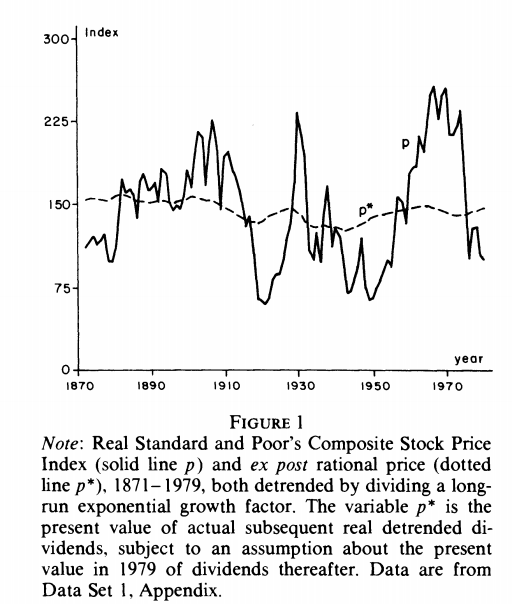
\includegraphics[width=\textwidth]{figures/slide09_pic3_Picture_5.png}\\[0.2em]
\footnotesize Shiller (1981)
\end{column}
\end{columns}
\end{frame}

% --- Slide 10: Aggregate stock market, ctd. ---
\begin{frame}{Aggregate Stock Market, ctd.}
\begin{itemize}
\item {\large \textbf{The equity premium puzzle}}
  \begin{itemize}
  \item The historical equity premium (5\%) is much higher than predicted by a simple rational, frictionless model with power utility preferences (Mehra and Prescott, 1985)
  \item The covariance of stock market returns with consumption growth is small
  \item The representative investor does not view the stock market as very risky, and requires a very low equity premium
  \end{itemize}
\end{itemize}
\end{frame}

% --- Slide 11: Section divider ---
\section{The Cross-Section of Stock Returns}

\begin{frame}{}
\vfill
\centering
{\Large \textbf{The Cross-Section of Stock Returns}}
\vfill
\end{frame}

% --- Slide 12: Cross-section, ctd. ---
\begin{frame}{The Cross-Section, ctd.}
\begin{columns}[T]
\begin{column}{0.50\textwidth}
\begin{itemize}
\item \textbf{Long-term reversal}
  \begin{itemize}
  \item A stock's cumulative return over the past 3--5 years negatively predicts its future return in the cross-section (De Bondt and Thaler, 1985)
  \item Rational hypothesis?
  \item What are other patterns that you notice?
  \end{itemize}
\end{itemize}
\end{column}
\begin{column}{0.48\textwidth}
\centering
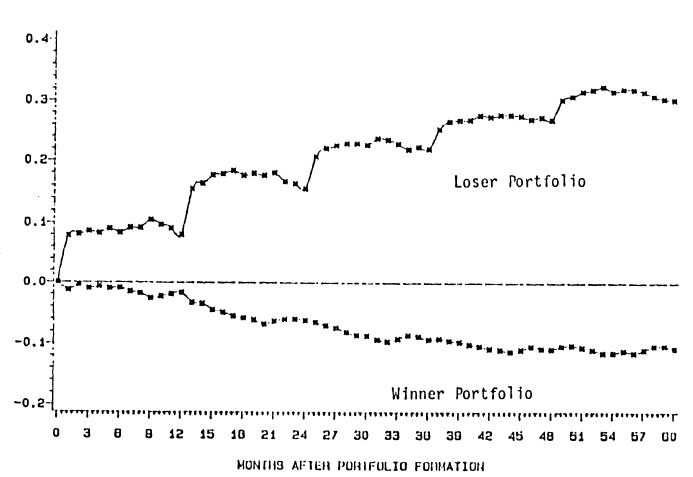
\includegraphics[width=\textwidth]{figures/slide12_pic3_Picture_1.jpg}
\end{column}
\end{columns}
\end{frame}

% --- Slide 13: Cross-section, ctd. ---
\begin{frame}{The Cross-Section, ctd.}
\begin{itemize}
\item \textbf{Momentum}
  \begin{itemize}
  \item A stock's $k$-month past return ($k$ between 3 and 12) positively predicts its future returns in the cross-section (Jegadeesh and Titman, 1993)
  \item Explaining both momentum and long-term reversal in a unified and parsimonious framework is an important challenge
  \end{itemize}
\end{itemize}
\vfill
\centering
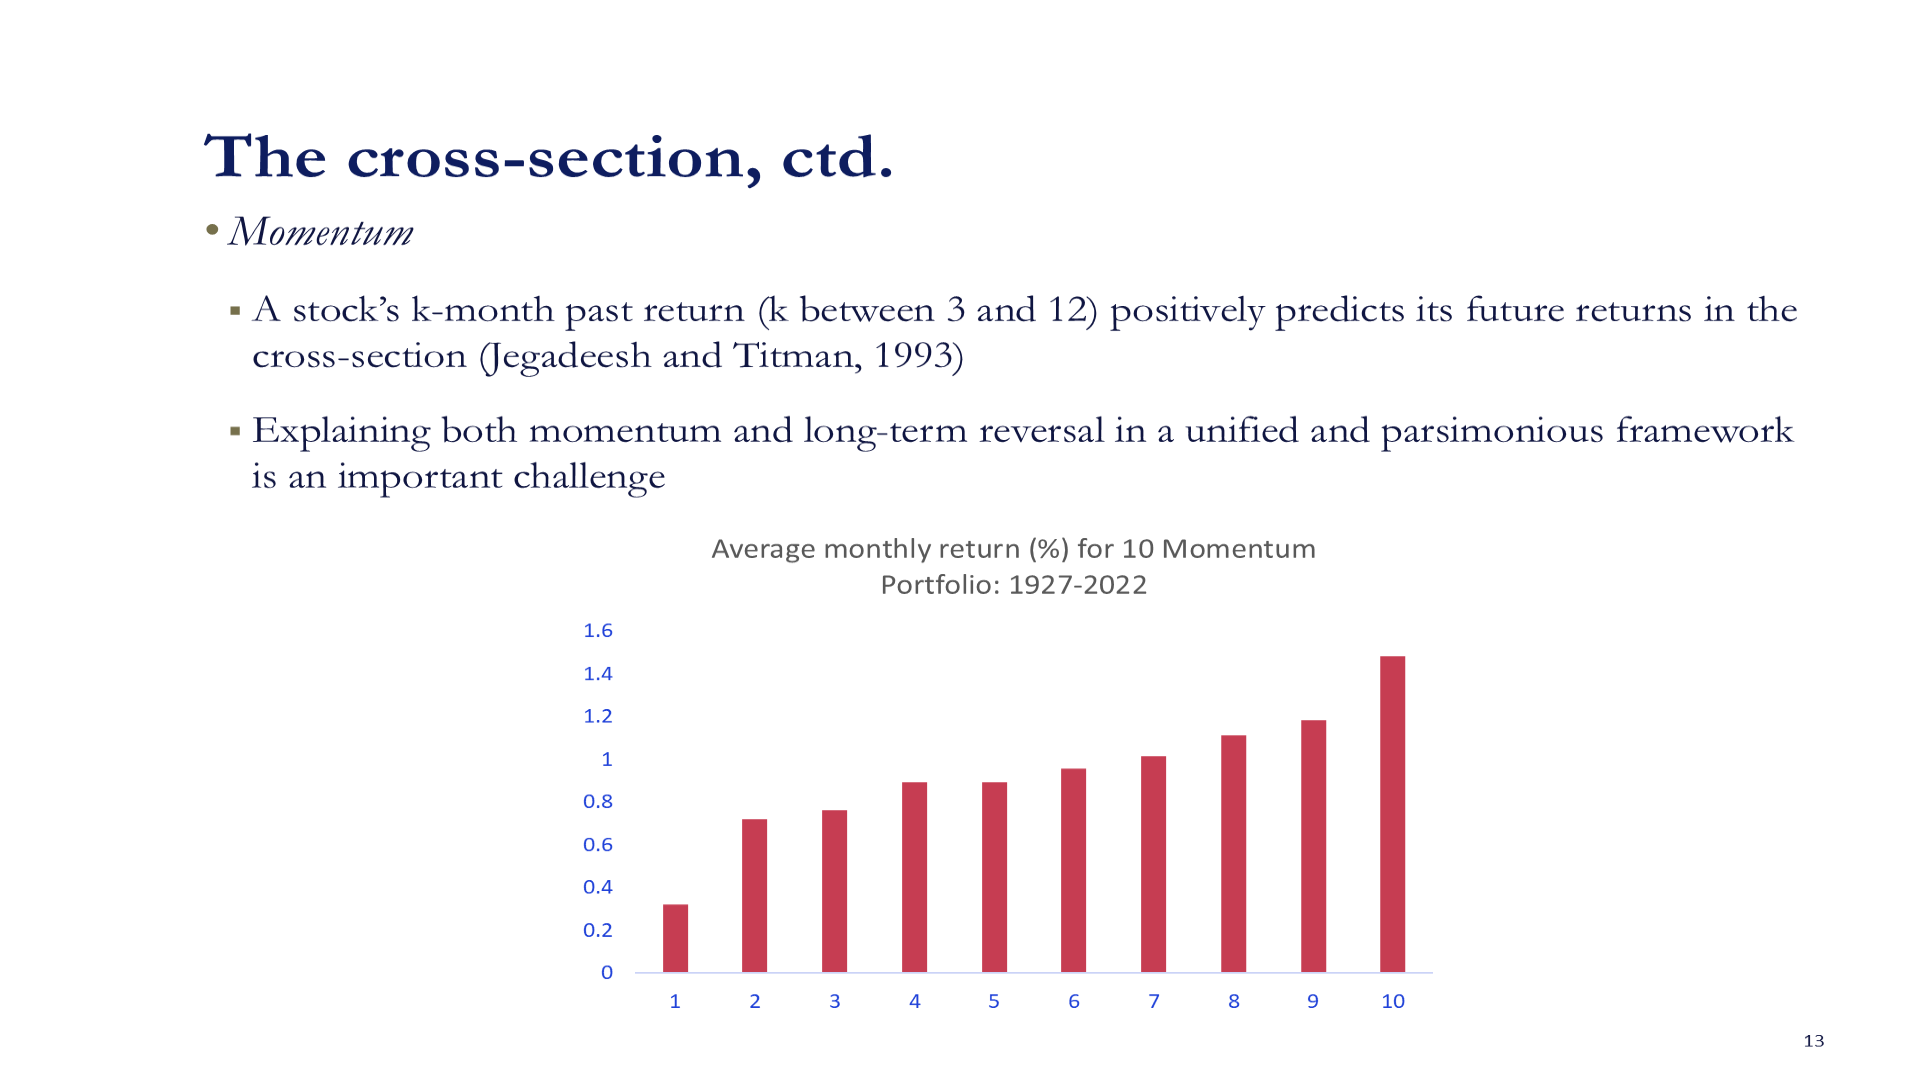
\includegraphics[width=0.55\textwidth]{figures/slide13_chart.png}
\end{frame}

% --- Slide 14: Cross-section, ctd. ---
\begin{frame}{The Cross-Section, ctd.}
\begin{columns}[T]
\begin{column}{0.50\textwidth}
\begin{itemize}
\item \textbf{Short-term reversal}
  \begin{itemize}
  \item A stock's return over the past week or month negatively predicts its future return in the cross-section (Jegadeesh, 1990; Lehmann, 1990)
  \item Could be explained by compensation for liquidity provision
  \item The returns of short-term reversal strategies in equity markets is highly predictable with the VIX index (Nagel, 2012)
  \end{itemize}
\end{itemize}
\end{column}
\begin{column}{0.48\textwidth}
\centering
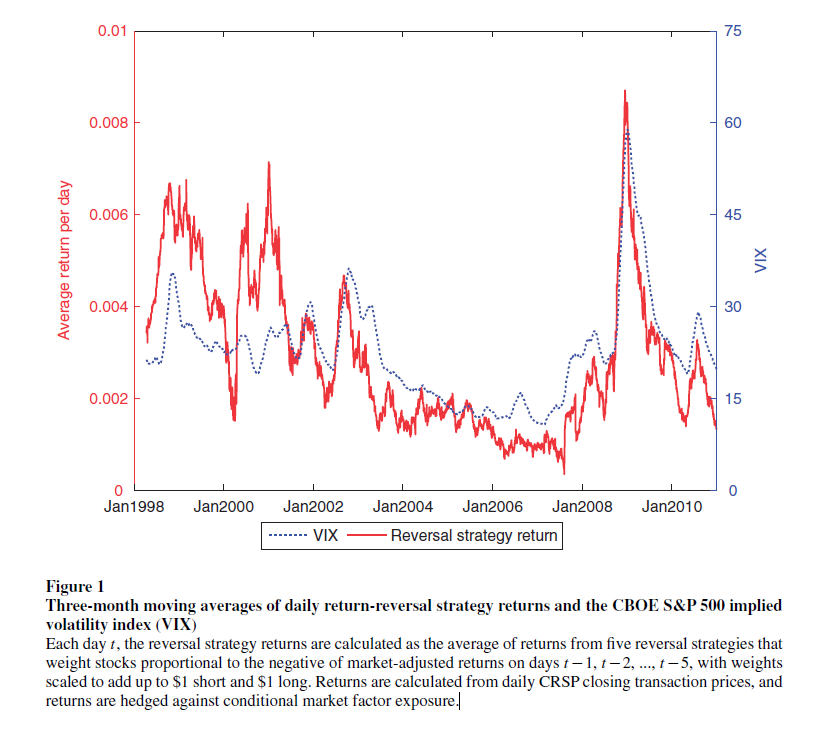
\includegraphics[width=\textwidth]{figures/slide14_pic2_Picture_6.png}\\[0.2em]
\footnotesize Nagel (RFS 2012)
\end{column}
\end{columns}
\end{frame}

% --- Slide 15: Cross-section, ctd. ---
\begin{frame}{The Cross-Section, ctd.}
\begin{itemize}
\item \textbf{The value premium}
  \begin{itemize}
  \item Ratios of fundamentals to price (B/M, E/P, CF/P) positively predict future returns
  \end{itemize}
\end{itemize}
\vfill
\centering
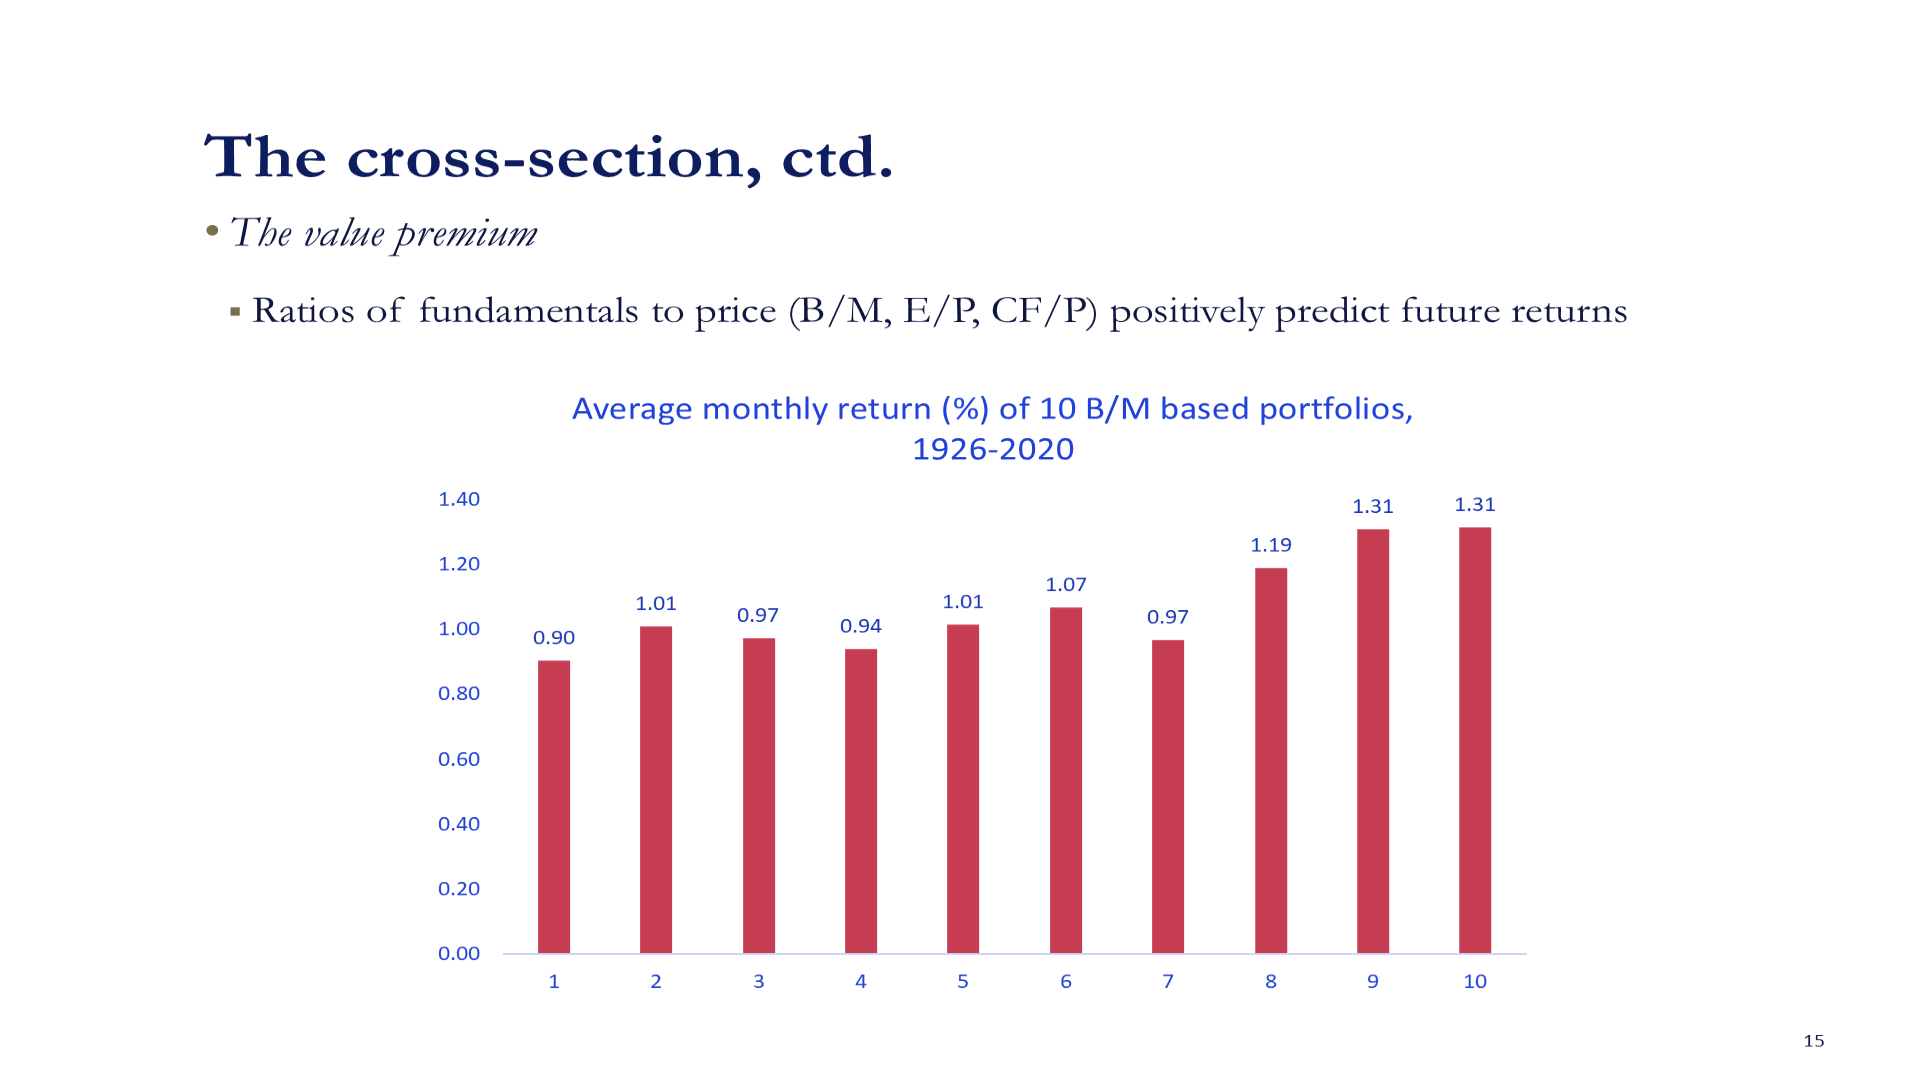
\includegraphics[width=0.7\textwidth]{figures/slide15_chart.png}
\end{frame}

% --- Slide 16: Cross-section, ctd. ---
\begin{frame}[shrink=5]{The Cross-Section, ctd.}
\begin{itemize}
\item The value and momentum effects also exist in other asset classes (Asness, Moskowitz, and Pedersen, 2013)
  \begin{itemize}
  \item Within most developed equity markets, across country equity indices, across government bond indices, across currencies, and across commodities
  \end{itemize}
\end{itemize}
\vfill
\centering
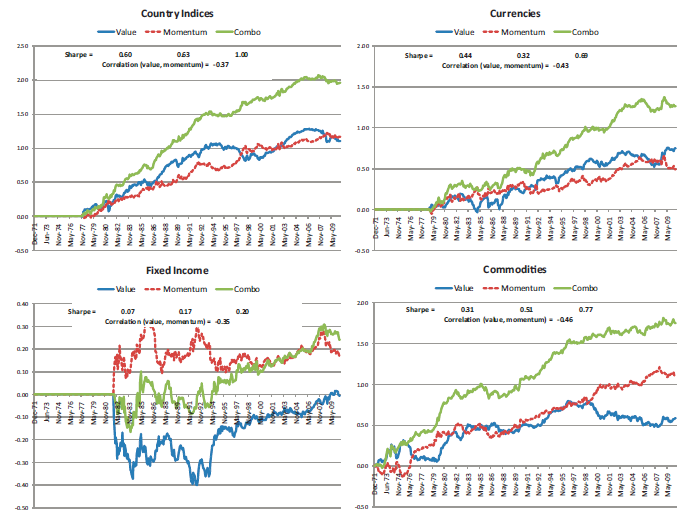
\includegraphics[width=0.5\textwidth]{figures/slide16_pic3_Picture_3.png}
\end{frame}

% --- Slide 17: Cross-section, ctd. ---
\begin{frame}{The Cross-Section, ctd.}
\begin{itemize}
\item \textbf{The issuance/repurchase anomaly}
  \begin{itemize}
  \item Firms that issue equity (IPO or SEO) subsequently do poorly, relative to a control group (Loughran and Ritter, 1995)
  \item Firms that repurchase equity subsequently do well, relative to a control group (Ikenberry, Lakonishok, and Vermaelen, 1995)
  \end{itemize}
\end{itemize}
\vfill
\centering
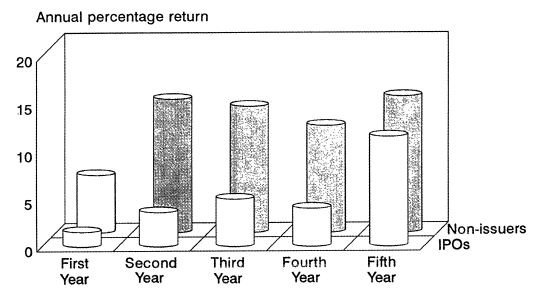
\includegraphics[width=0.38\textwidth]{figures/slide17_pic4_Picture_6.jpg}
\hspace{0.5em}
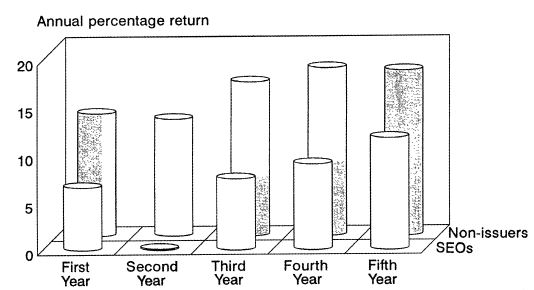
\includegraphics[width=0.38\textwidth]{figures/slide17_pic3_Picture_5.jpg}
\end{frame}

% --- Slide 18: Cross-section, ctd. ---
\begin{frame}{The Cross-Section, ctd.}
\begin{itemize}
\item \textbf{The asset growth / investment anomaly}
  \begin{itemize}
  \item Firms that grow assets more quickly or invest more have lower risk-adjusted return (Titman, Wei, and Xie, 2004; Cooper, Gulen, and Schill, 2008)
  \end{itemize}
\end{itemize}
\vfill
\centering
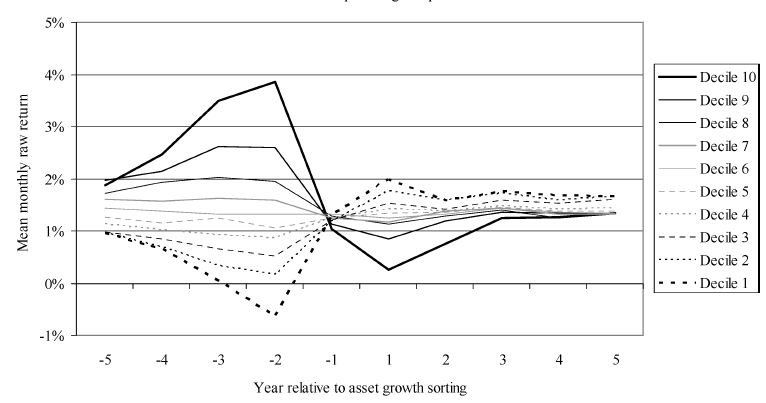
\includegraphics[width=0.70\textwidth]{figures/slide18_pic3_Picture_2.jpg}
\end{frame}

% --- Slide 19: Cross-section, ctd. ---
\begin{frame}{The Cross-Section, ctd.}
\begin{itemize}
\item \textbf{The Profitability anomaly:} more profitable firms (quintile 5) earn higher returns than less profitable firms (quintile 1)
\item Profitability is related to a broad set of \emph{Quality} characteristics
  \begin{itemize}
  \item Asness, Frazzini, \& Pedersen (2019) suggest a multiple dimensional gauge of quality: profitability, recent growth in profits, low return and earnings volatility, and low leverage
  \end{itemize}
\end{itemize}
\vfill
\centering
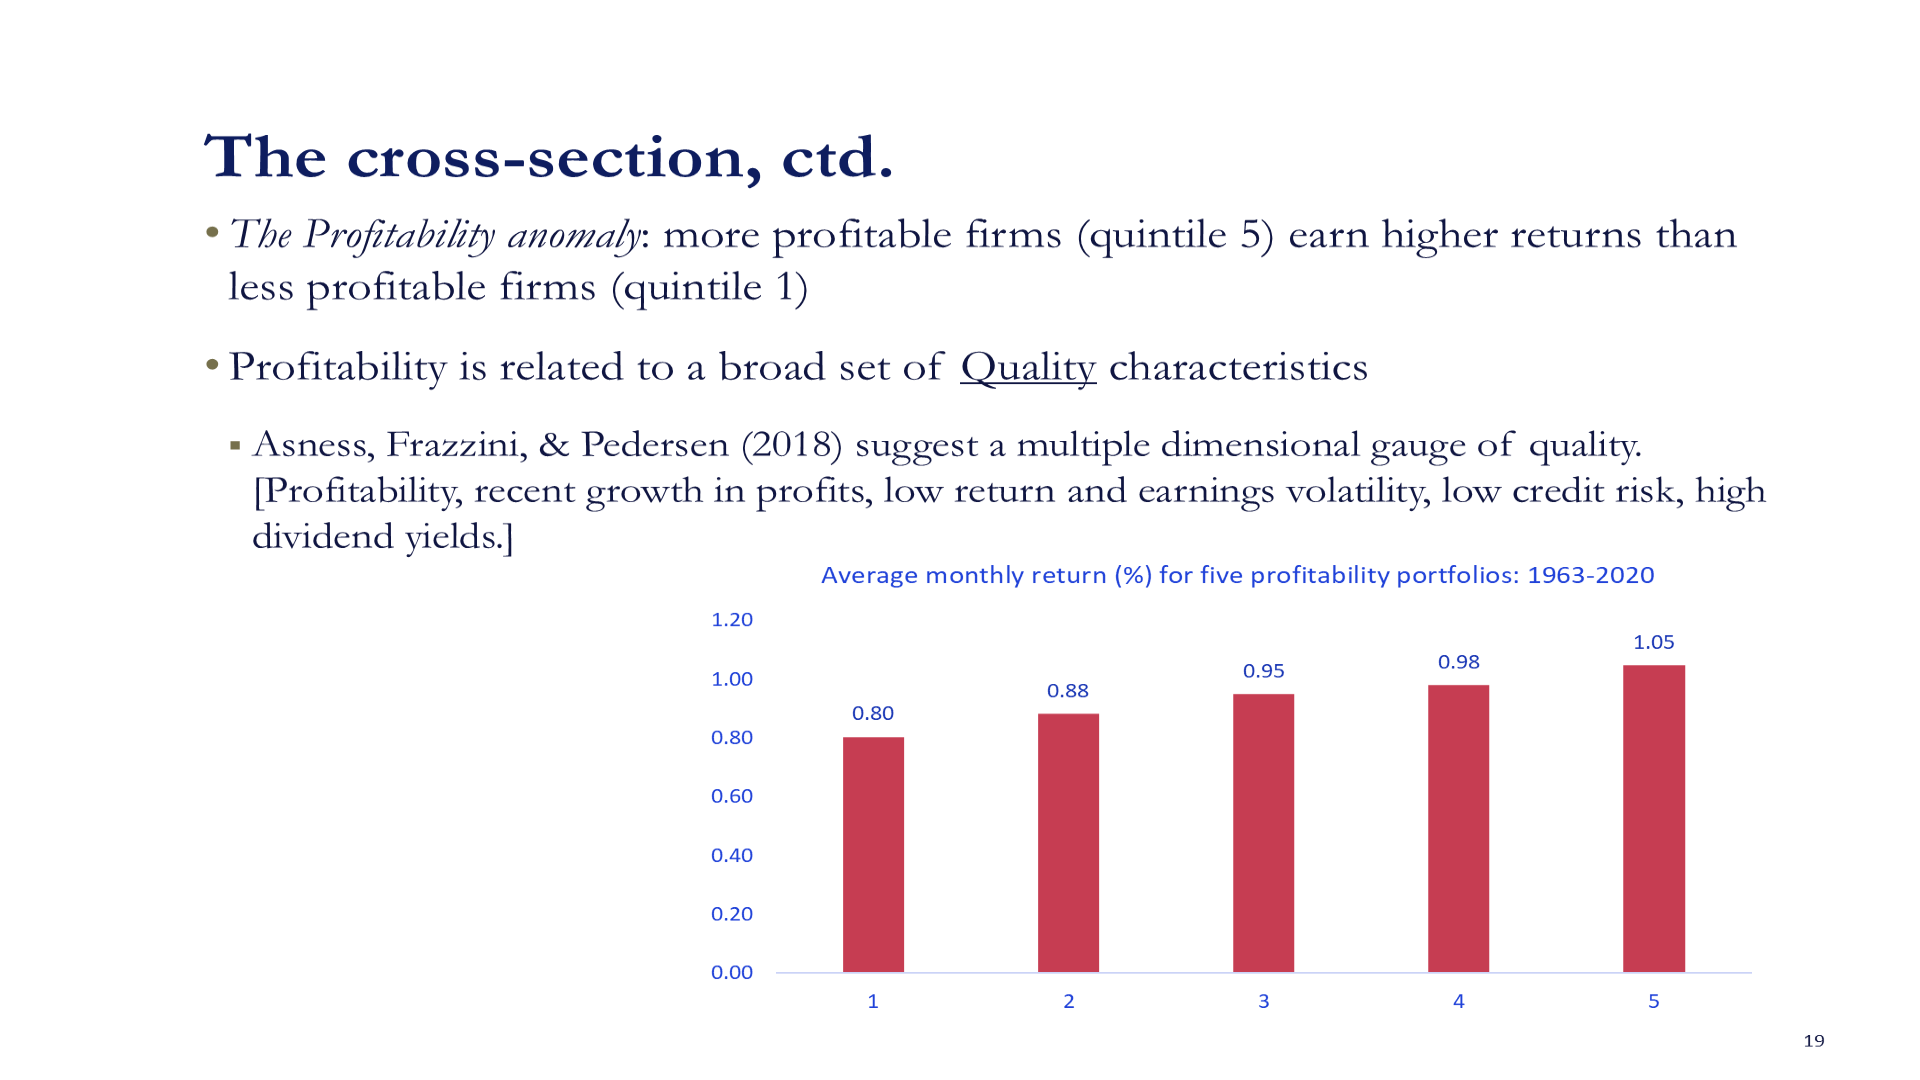
\includegraphics[width=0.60\textwidth]{figures/slide19_chart.png}
\end{frame}

% --- Slide 20: Cross-section, ctd. ---
\begin{frame}{The Cross-Section, ctd.}
\begin{itemize}
\item \textbf{The financial distress anomaly}
  \begin{itemize}
  \item Financially distressed stocks earn lower alphas (Campbell, Hilscher, and Szilagyi, 2008)
  \end{itemize}
\end{itemize}
\vfill
\centering
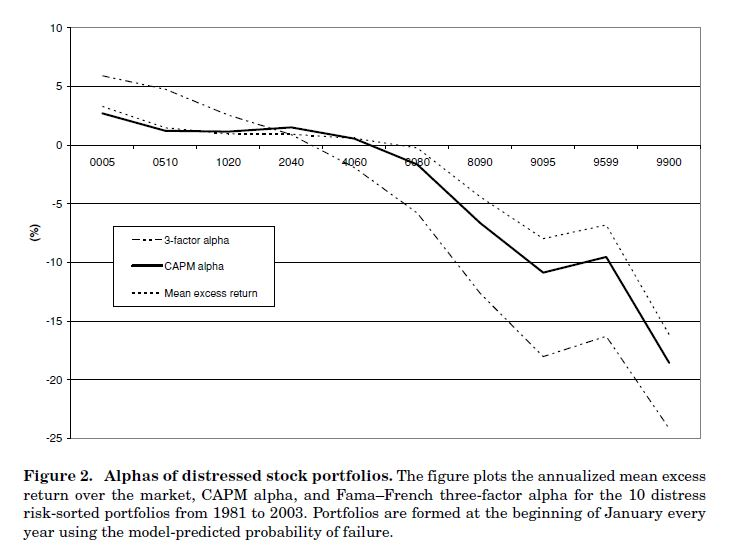
\includegraphics[width=0.50\textwidth]{figures/slide20_pic3_Picture_5.jpg}
\end{frame}

% --- Slide 21: Cross-section, ctd. ---
\begin{frame}[shrink=5]{The Cross-Section, ctd.}
\begin{columns}[T]
\begin{column}{0.50\textwidth}
\begin{itemize}
\item \textbf{Post-earnings announcement drift}
  \begin{itemize}
  \item The surprise in a firm's most recent earnings announcement positively predicts future returns
  \end{itemize}
\item \textbf{Other related findings:}
  \begin{itemize}
  \item The revision in analysts' consensus earnings forecast/recommendations positively predicts future returns
  \end{itemize}
\end{itemize}
\end{column}
\begin{column}{0.40\textwidth}
\centering
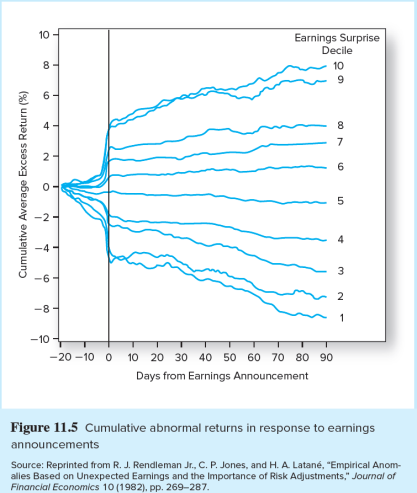
\includegraphics[width=\textwidth]{figures/slide21_pic3_Picture_2.png}
\end{column}
\end{columns}
\end{frame}

% --- Slide 22: Cross-section, ctd. ---
\begin{frame}{The Cross-Section, ctd.}
\begin{columns}[T]
\begin{column}{0.50\textwidth}
\begin{itemize}
\item \textbf{Idiosyncratic volatility puzzle}
  \begin{itemize}
  \item Stocks with higher idiosyncratic volatility have lower alphas (Ang et al., 2006)
  \end{itemize}
\end{itemize}
\end{column}
\begin{column}{0.48\textwidth}
\centering
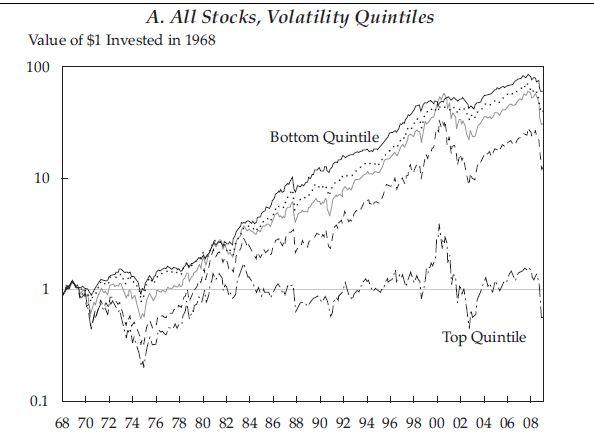
\includegraphics[width=\textwidth]{figures/slide22_pic3_Picture_3.jpg}\\[0.2em]
\footnotesize Baker, Bradley and Wurgler (2011, FAJ)
\end{column}
\end{columns}
\end{frame}

% --- Slide 23: Cross-section, ctd. ---
\begin{frame}{The Cross-Section, ctd.}
\begin{columns}[T]
\begin{column}{0.50\textwidth}
\begin{itemize}
\item \textbf{The Beta Anomaly}
  \begin{itemize}
  \item Stocks with higher betas have similar raw return and lower CAPM alpha than low beta stocks
  \item In other words, the empirical SML is too flat compared to that predicted by CAPM
  \end{itemize}
\end{itemize}
\end{column}
\begin{column}{0.48\textwidth}
\centering
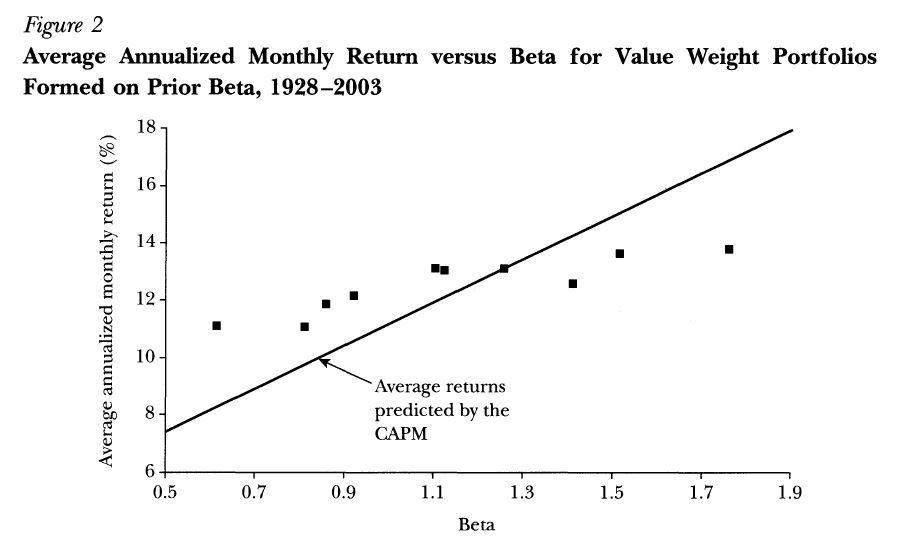
\includegraphics[width=\textwidth]{figures/slide23_pic3_Picture_3.jpg}\\[0.2em]
\footnotesize Fama and French (2004)
\end{column}
\end{columns}
\end{frame}

% --- Slide 24: Cross-section, ctd. ---
\begin{frame}{The Cross-Section, ctd.}
\begin{itemize}
\item Similar findings in other countries and other asset classes (Frazzini and Pedersen, 2014)
\item \textbf{Betting against beta} is highly profitable
\end{itemize}
\vfill
\centering
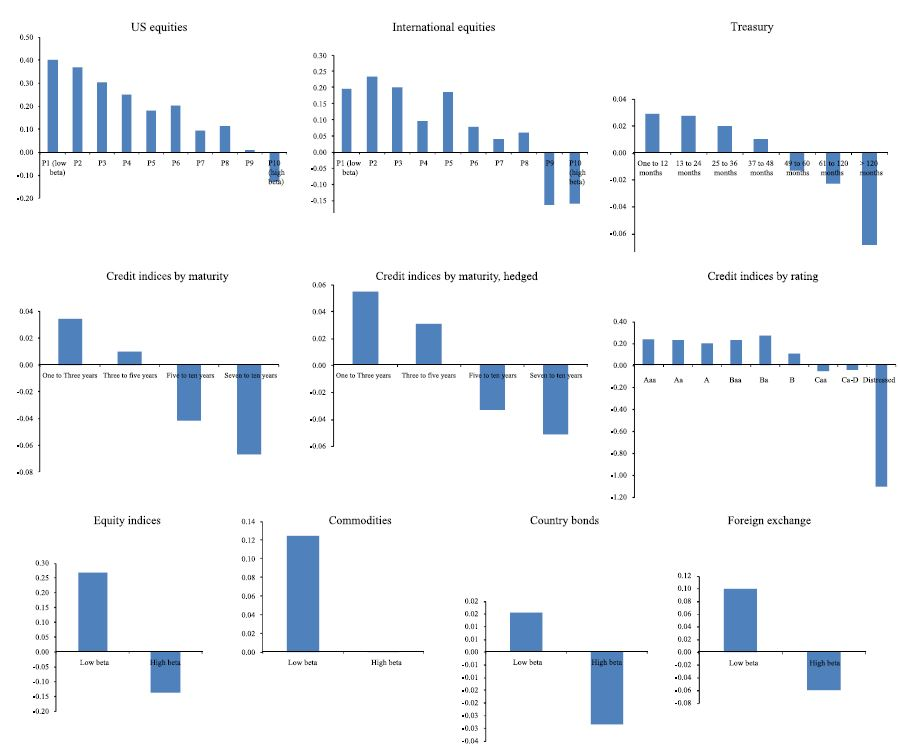
\includegraphics[width=0.50\textwidth]{figures/slide24_pic3_Picture_1.jpg}
\end{frame}

% --- Slide 25: Cross-section, ctd. ---
\begin{frame}{The Cross-Section, ctd.}
\centering
\textbf{Firm-level characteristics with predictive power for stock returns in the cross-section}
\vfill
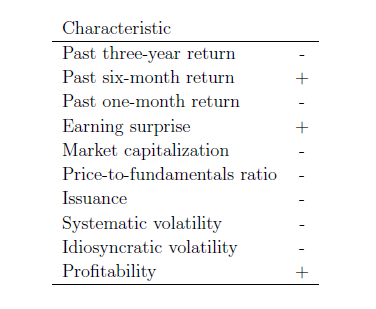
\includegraphics[width=0.55\textwidth]{figures/slide25_pic3_Picture_6.png}
\end{frame}

% --- Slide 26: Bubbles ---
\section{Bubbles}

\begin{frame}{Bubbles}
\footnotesize
\begin{itemize}
\item Situations where, for a significant period of time, an asset trades at a price that appears to be substantially higher than its rational/frictionless price
\item Bubbles appear to exhibit following characteristics:
  \begin{itemize}
  \item[\textit{(i)}] The price of an asset rises sharply over some period of time and then declines, reversing much of the rise
  \item[\textit{(ii)}] During the price rise, there are many reports in the media and from sophisticated investors that the asset is overvalued
  \item[\textit{(iii)}] As the price of the asset rises and reaches its peak, there is an abnormally high volume of trading in the asset
  \item[\textit{(iv)}] During the episode, many investors have highly extrapolative expectations about returns, in that their expectation about the asset's future return rises with the asset's past return
  \item[\textit{(v)}] During the price rise, some sophisticated investors increase their exposure to the asset
  \item[\textit{(vi)}] In the early stages of the price rise, there is positive news about the asset's future fundamental
  \end{itemize}
\end{itemize}
\end{frame}

% --- Slide 27: Famous Bubbles ---
\begin{frame}[shrink=5]{Famous Bubbles in History}
\vfill
\centering
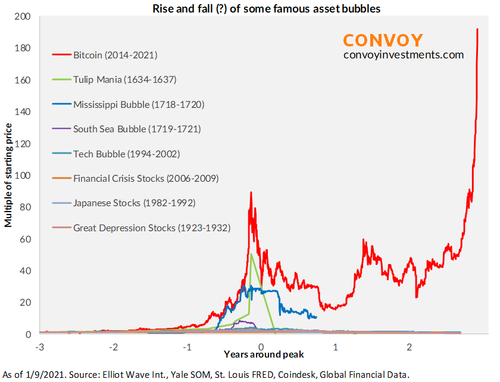
\includegraphics[width=0.6\textwidth]{figures/slide27_pic2_Picture_5.png}
\vfill
\end{frame}

% --- Slide 28: Bubbles, ctd. ---
\begin{frame}{Bubbles, ctd.}
\begin{columns}[T]
\begin{column}{0.50\textwidth}
\begin{itemize}
\item Bubbles tend to be accompanied by very high trading volume (Hong and Stein, 2007)
\item And sophisticated traders often ``ride'' the bubble (Brunnermeier and Nagel, 2004)
\item Understanding bubbles is an important challenge
  \begin{itemize}
  \item Their collapse can trigger severe economic downturns
  \end{itemize}
\end{itemize}
\end{column}
\begin{column}{0.48\textwidth}
\centering
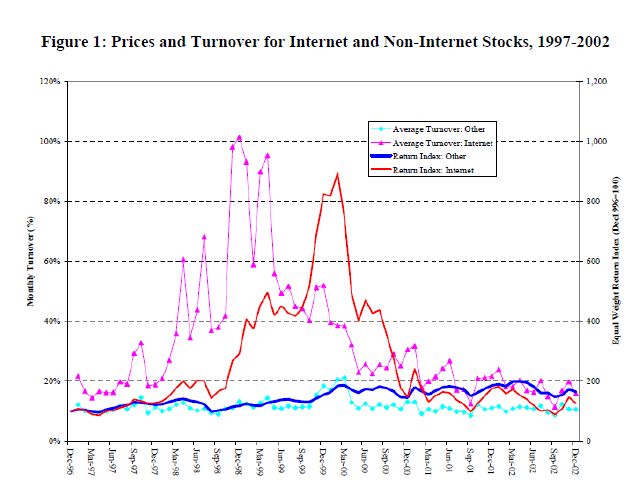
\includegraphics[width=\textwidth]{figures/slide28_pic2_Picture_6.png}
\end{column}
\end{columns}
\end{frame}

% --- Slide 29: Investor Trading ---
\section{Investor Trading and Portfolio Choice}

\begin{frame}{Investor Trading and Portfolio Choice}
\begin{itemize}
\item \textbf{Individual investors}
  \begin{itemize}
  \item Non-participation
  \item Buying high and selling low
  \item Under-diversification
  \item Excessive trading
  \item Sell winners too quickly and hold on to losers for too long (``Disposition effect'')
  \end{itemize}
\item \textbf{Institutional investors}
  \begin{itemize}
  \item Average performance
  \item Trade against anomalies
  \item Sentiment-driven trading
  \end{itemize}
\end{itemize}
\end{frame}

% --- Slide 30: Individual Investors ---
\section{Individual Investors}

\begin{frame}{Individual Investors}
\begin{itemize}
\item \textbf{Non-participation}
  \begin{itemize}
  \item Historically, most U.S.\ households held no stock at all
    \begin{itemize}
    \item E.g.\ in 1984, only 28\% of households held any stock (Mankiw and Zeldes, 1991)
    \end{itemize}
  \item But a simple rational, frictionless model of portfolio choice predicts that all households should have at least some stock market exposure
  \end{itemize}
\item \textbf{Rational hypotheses?}
  \begin{itemize}
  \item Fixed transaction costs in participating in stock market
  \item Correlated background risk including labor income and real estate
  \end{itemize}
\end{itemize}
\end{frame}

% --- Slide 31: Individual Investors, ctd. ---
\begin{frame}{Individual Investors, ctd.}
\begin{itemize}
\item \textbf{Buying high, selling low}
  \begin{itemize}
  \item Investors' actual historical returns are much lower than the buy-and-hold returns (Dichev, 2007)
  \end{itemize}
\end{itemize}
\vfill
\centering
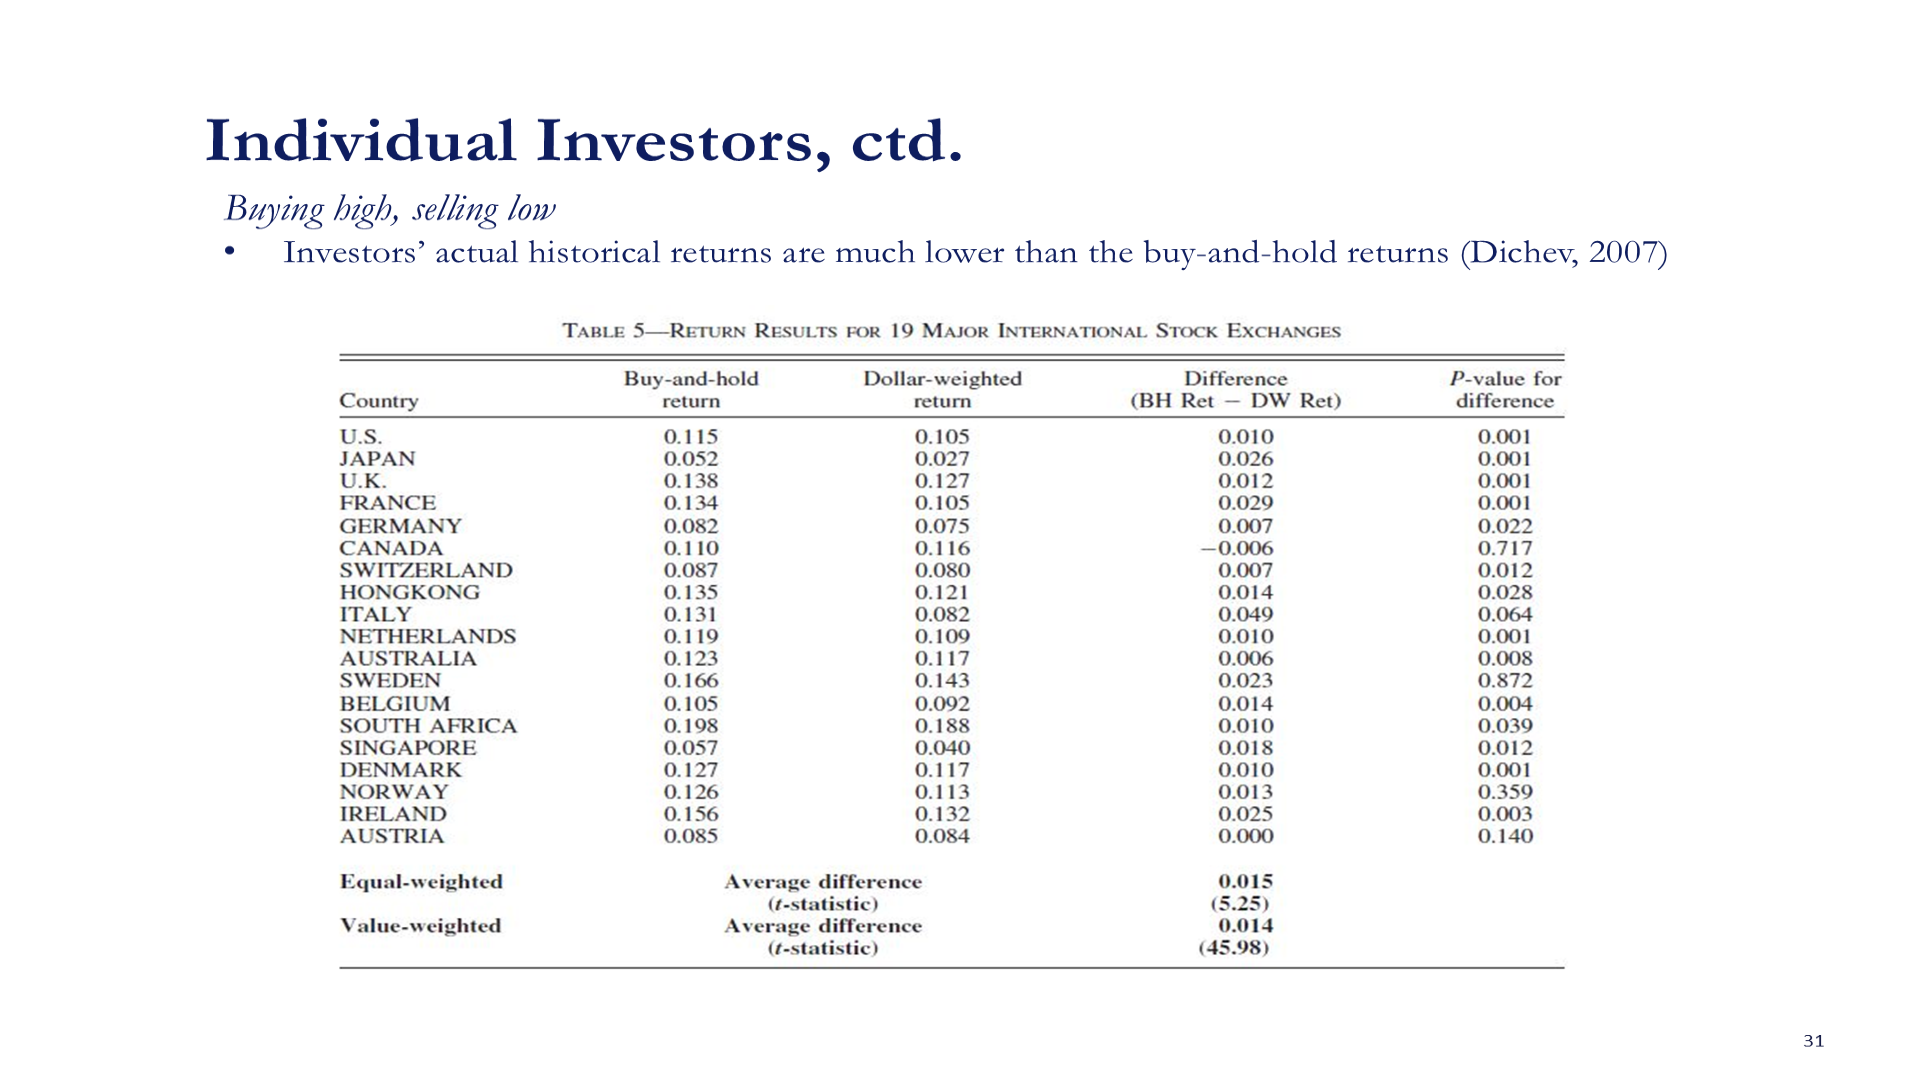
\includegraphics[width=0.65\textwidth]{figures/slide31_chart.png}
\end{frame}

% --- Slide 32: Individual Investors, ctd. ---
\begin{frame}[shrink=10]{Individual Investors, ctd.}
\footnotesize
\begin{itemize}
\item Many households seem to be less diversified than recommended by traditional models of portfolio choice
\item \textbf{Under-diversification: Home bias}
  \begin{itemize}
  \item Investors allocate a surprisingly large fraction of their equity holdings to domestic equity
  \item In 1989, U.S., U.K., and Japanese households invested 94\%, 82\% and 98\% of their equity holdings in domestic equity (French and Poterba, 1991)
  \end{itemize}
\item \textbf{Under-diversification: Local bias}
  \begin{itemize}
  \item The typical U.S.\ household has about 30\% of its portfolio invested in stocks headquartered within a 250-mile radius of the family's home
  \end{itemize}
\item \textbf{Rational explanations?}
  \begin{itemize}
  \item Information advantage in local firms
  \item Mixed evidence for this explanation (Ivkovic and Weisbenner, 2005; Seasholes and Zhu, 2010)
  \end{itemize}
\end{itemize}
\end{frame}

% --- Slide 33: Individual Investors, ctd. ---
\begin{frame}[shrink=10]{Individual Investors, ctd.}
\begin{columns}[T]
\begin{column}{0.58\textwidth}
\begin{itemize}
\item \textbf{Under-diversification: Ownership of few individual stocks}
  \begin{itemize}
  \item Curcuru et al.\ (2004) report that, in 1989, 30\% of U.S.\ equity-owning households allocated more than 50\% of their equity exposure to fewer than 10 stocks
  \end{itemize}
\item \textbf{Under-diversification: Own-company stock}
  \begin{itemize}
  \item Benartzi (2001) reports that, in a sample of 154 retirement plans, people allocated 23\% of their discretionary contributions to own-company stock
  \end{itemize}
\end{itemize}
\end{column}
\begin{column}{0.30\textwidth}
\centering
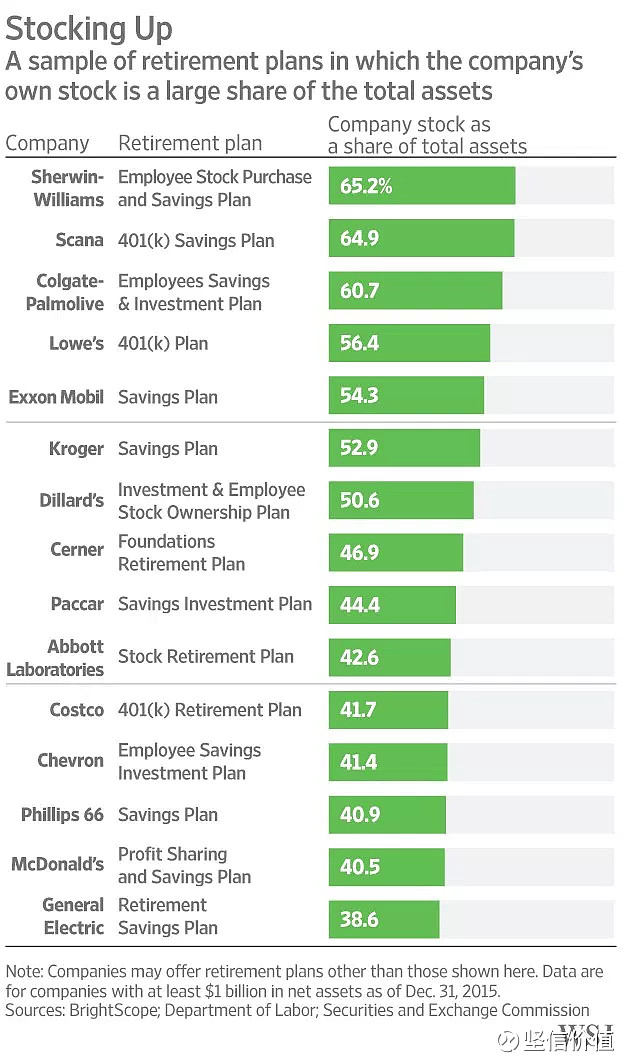
\includegraphics[width=\textwidth]{figures/slide33_pic0_Picture_5.jpg}
\end{column}
\end{columns}
\end{frame}

% --- Slide 34: Individual Investors, ctd. ---
\begin{frame}{Individual Investors, ctd.}
\begin{itemize}
\item \textbf{Excessive trading}
  \begin{itemize}
  \item Using data on 66,465 households with accounts at a large discount brokerage firm, Barber and Odean (2000) find that investors who trade more earn lower return in stock market
  \end{itemize}
\end{itemize}
\vfill
\centering
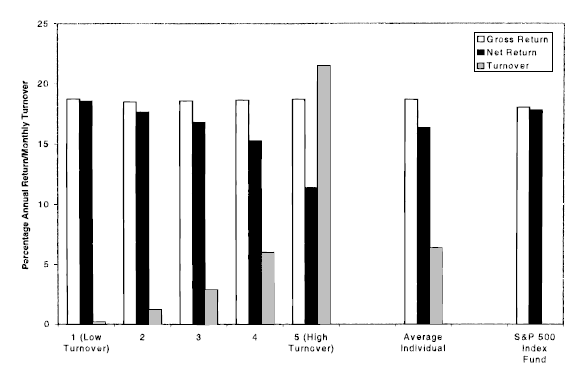
\includegraphics[width=0.55\textwidth]{figures/slide34_pic3_Picture_2.png}
\end{frame}

% --- Slide 35: Individual Investors, ctd. ---
\begin{frame}{Individual Investors, ctd.}
\begin{itemize}
\item \textbf{Disposition effect}
  \begin{itemize}
  \item Individual investors have a greater tendency to sell stocks trading at a gain relative to purchase price, rather than at a loss (Odean, 1998)
  \end{itemize}
\item Tested by Odean (1998) using the following hypothesis on investor behavior:
\item Proportion of Gains Realized (PGR) $>$ Proportion of Losses Realized (PLR)
\end{itemize}
\vfill
\centering
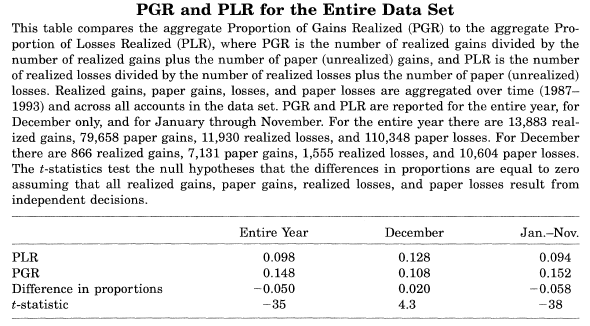
\includegraphics[width=0.50\textwidth]{figures/slide35_pic3_Picture_2.png}
\end{frame}

% --- Slide 36: Individual Investors, ctd. ---
\begin{frame}{Individual Investors, ctd.}
\begin{itemize}
\item A similar effect is present among mutual fund managers (Frazzini, 2006) and also in the housing market (Genesove and Mayer, 2001)
\item The most obvious potential explanations, e.g.\ informed trading, fail to capture important features of the data
  \begin{itemize}
  \item Subsequent return of winners that people sell is higher than that of losers they hold on to
  \end{itemize}
\item The disposition effect is more pronounced among less sophisticated investors (Dhar and Zhu, 2006)
\end{itemize}
\end{frame}

% --- Slide 37: Individual Investors, ctd. ---
\begin{frame}{Individual Investors, ctd.}
\begin{itemize}
\item \textbf{Trading against anomalies---forecast returns}
\item Firms and short sellers tend to be the smart money---both sell stocks with \textbf{low-forecasted returns}
\end{itemize}
\vfill
\centering
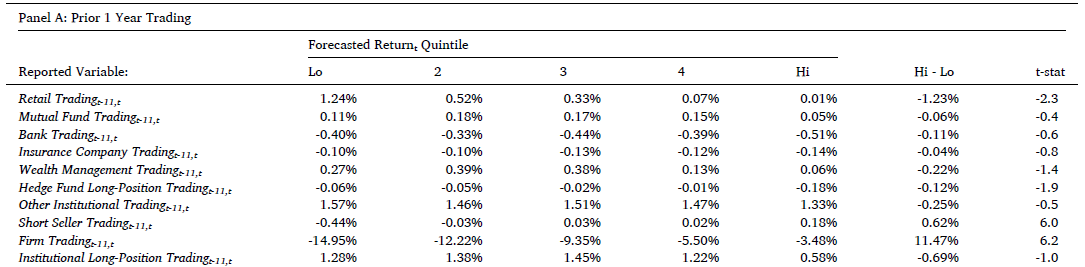
\includegraphics[width=0.85\textwidth]{figures/slide37_pic3_Picture_6.png}\\[0.2em]
\footnotesize McLean, Pontiff and Reilly (JFE 2025)
\end{frame}

% --- Slide 38: Institutional Investors ---
\section{Institutional Investors}

\begin{frame}{Institutional Investors}
\begin{itemize}
\item \textbf{Average performance}
  \begin{itemize}
  \item A basic frictionless model with skilled managers and rational investors (Berk and Green, 2004) predicts that:
    \begin{itemize}
    \item Managers' gross alpha will be positive, on average
    \item And their net alpha will be zero, on average
    \end{itemize}
  \item In practice, the gross alpha of mutual funds appears to be positive, but not substantially so
  \item Does this suggest there is no mispricing?
    \begin{itemize}
    \item No one earns abnormal profit equivalent to price is correct?
    \end{itemize}
  \end{itemize}
\end{itemize}
\end{frame}

% --- Slide 39: Institutional Investors, ctd. ---
\begin{frame}{Institutional Investors, ctd.}
\begin{itemize}
\item \textbf{Trading against anomalies}
  \begin{itemize}
  \item Lewellen (2011) finds that institutional investors in aggregate essentially hold the market portfolio, with no discernible tilt to take advantage of well-known stock return anomalies
  \item Edelen, Ince and Kadlec (2016) find more striking result that institutions have a strong tendency to buy overvalued stocks during portfolio formation
  \item Hedge funds and institutions with high turnover seem to exploit anomalies more than other institutions
  \end{itemize}
\end{itemize}
\end{frame}

% --- Slide 40: Institutional Investors, ctd. ---
\begin{frame}{Institutional Investors, ctd.}
\vfill
\centering
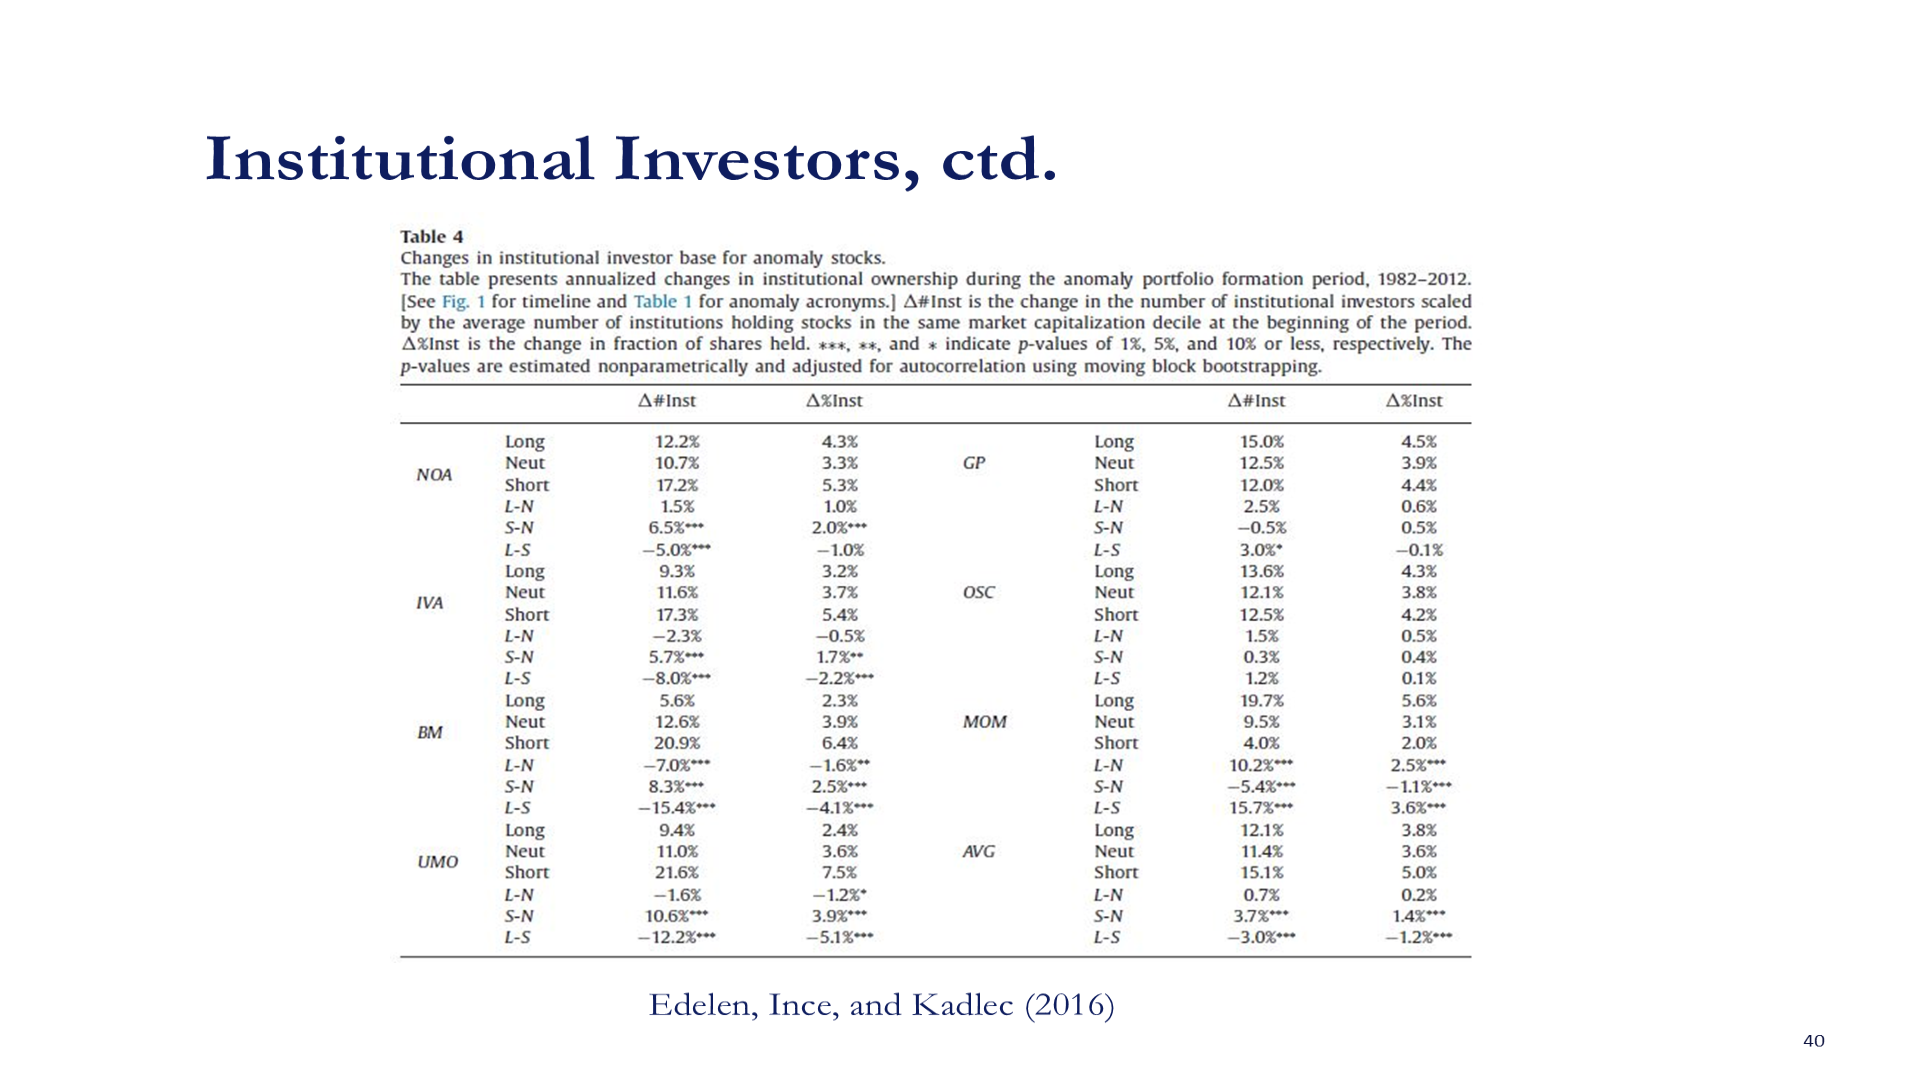
\includegraphics[width=0.65\textwidth]{figures/slide40_chart.png}\\[0.3em]
\footnotesize Edelen, Ince, and Kadlec (2016)
\vfill
\end{frame}

\end{document}
